\chapter{Introduction}

\section{Physics Motivation}

The existence of additional $U(1)$ gauge symmetries of nature are ubiquitous in
several Beyond the Standard Model (BSM) theories [].  As Holdom 
\cite{holdom1986} realized in the by mid eighties, in a theory with 
$U(1)_Y \times U(1)'$, the gauge term of the Lagrangian can be written as 
\begin{equation}
    \mathcal{L}_{\text{gauge}} = - \frac{1}{4} F_Y^{\mu \nu}F_{Y, \mu \nu}
                          - \frac{1}{4} F'^{\mu \nu}F'_{\mu \nu}
                          + \frac{1}{2} \epsilon F'^{\mu \nu} F_{Y, \mu \nu}
    \label{eqn:l_gauge}
\end{equation}
%the associated gauge boson (heavy photon,
%dark photon or $A'$) can couple to the SM photon through the ``kinetic mixing''
%interaction
where $F'_{\mu \nu} = \partial_{\mu}A'_{\nu} - \partial_{\nu}A'_{\mu}$ 
($F^{\mu \nu}_{Y} = \partial^{\mu}A^{\nu} - \partial^{\nu}A^{\mu}$) is the
field strength tensor of the heavy photon (SM hypercharge) and $\epsilon$ is a
dimensionless coupling constant.  Decoupling of the fields can be done by 
redefining the $A$ gauge field as 
\begin{equation}
    A_{\mu} \rightarrow A_{\mu} - \epsilon A'_{\mu}.
\end{equation}
The results in the diagnolization of \ref{eqn:l_gauge} as
\begin{equation}
    \mathcal{L}_{\text{gauge}} = - \frac{1}{4} F_Y^{\mu \nu}F_{Y, \mu \nu}
                          - \frac{1}{4} F'^{\mu \nu}F'_{\mu \nu}
                          + \frac{1}{2} \epsilon F'^{\mu \nu} F_{Y, \mu \nu}.
\end{equation}
However, the redefinition of the field also affects the interaction term of 
the Lagrangian
\begin{equation}
    \mathcal{L}_{int} 
\end{equation}
This, in turn, induces an effective coupling between the electromagnetic current
and the heavy photon field as 
\begin{equation}
    \mathcal{L}_{int} = \epsilon A'^{\mu}J_{\mu}^{EM}
\end{equation}
As explained below, this interaction can be exploited to search for heavy 
photons.

Several theories have envisioned scenarios generating 
$\epsilon \sim 10^{-6} - 10^{-2}$.

\section{Motivations for a Heavy Photon from Dark Matter}

Although the existence of dark photon can be motivated independently of a link
to dark matter, their possible interaction can provide a portal that would allow
probing of a dark sector which may contain a rich zoo of dark particles.  
Furthermore, Several recently observed astrophysical anamolies can be 
resolved if dark matter interactions are mediated by an $A'$.

The exploration of a link between an $A'$ and dark matter began in 200* after
the observation of an excess in the positron spectrum by the PAMELA experiment
\cite{}.

\section{Current Limits on Heavy Photons}

\subsection{Electorn Beam Dump Experiments}

Electron beam dump experiments make use of a high intensity beam ``dumped'' onto
a thick ($\sim$ cm) target to produce heavy photons through a process analogous
to photon bremstrahlung.  The thickness of the targets and the high luminosities
allow such experiments to be sensitive to heavy photons with small couplings 
which tend to travel considerable distances before decaying.  

Several beam dump experiments took place over the last decade. These include 
%E137 \cite{PhysRevD.38.3375} and E141 \cite{PhysRevLett.59.755} conducted at 
SLAC, 


\begin{figure}[t]
    \centering
    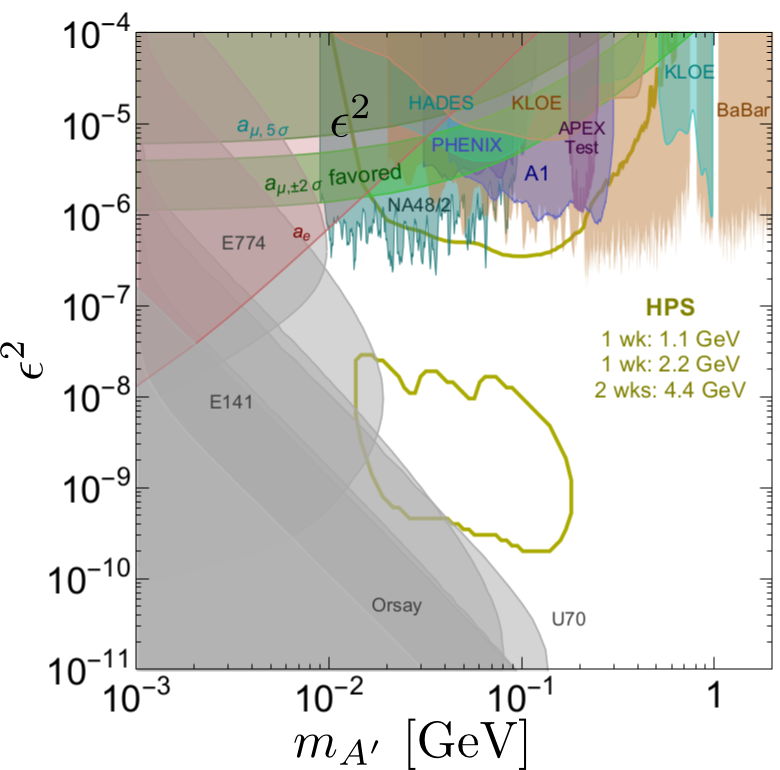
\includegraphics[width=0.9\textwidth]{images/ap_current_limits.png}
    \caption{Current limits on heavy photons.}
    \label{fig:svt_layout_render}
\end{figure}
